% Architecture Description and system specifications
% 	* Multisensor IMS		
%		* Processing Stages
%		* Fusion approaches		
%	* Validation approaches
%		* Transportation and Traffic Simulations
%			* Simulators Classification
%		* Intersection monitoring Datasets
%			* POSSi Dataset
%			* KoPER Dataset
%	* Architecture proposal

\chapter [Architecture Description and System Specification]{Architecture Description and System Specification}
\chaptermark {System Description}

Although several types of sensors are used for intersection monitoring and supervision, the use of cameras, lasers and lidars has increased due to advances in sensors manufacturing and computing capabilities. Such enhancements allows to deploy more of those types of sensors per scenario and it is required to define some processing stages from raw data capture through decision and control stages. It is also needed to test and validate the developments prior to a real and full functional implementation. The first part of this chapter describes the main stages in a intersection management system, from data preprocessing to situation assesment. Then, two validation tools for IMS applications are described, simulation models and datasets. And finally, the proposed architecture for the implementation of an IMS system is presented.

\section{Multisensor IMS}

Multicamera and multilasers monitoring systems offer more information about environment that can be merged to provide a better representation of the whole scene, detect with more accuracy the objects in the intersection, and prevent possible incidents. For designing a single-sensor or multi-sensor IMS, there are some basic processing stages to have into account. In the case of a multisensor system, it is also required to analyse and determine which is the better fusion approach to use and in which of the processing stages this fusion should be performed, in order to get better results than a single-sensor based system.

\subsection{Processing Stages}

In the designing of an IMS, there are four main stages that have to be performed from the data source to final output: preprocessing, feature analysis, pattern recognition and situation assessment. The aim of the first stage is to extract data of interest from the raw sensor information, using filtering to remove noise and irrelevant data, and background subtraction techniques to get the foreground of the scene. Spatial-temporal alignment of data is also performed in this stage. In the second stage, the objective is to identify elements within the foreground and extract relevant features of them. The third stage receives the set of features from the previous stage and performs recognition and classification tasks. Also, tracking and prediction of objects' state is performed based on historic information. In the fourth stage, object behaviour and inter-objects interaction are analysed to identify context and detect situations or events of interest. This output could be delivered to an optional fifth stage of decision and control, to a human operator, or to a traffic agent or institution, to take immediate actions on traffic control, issue traffic tickets, warn drivers about possible incidents or improve transportation policies in a long-term basis. In figure \ref{proc_stages}, previously described stages are depicted, including a list of common tasks performed at each of these stages and also it is shown how the data volume is reduced while data meaning increases in the last stages. 

\begin{figure}[ht!]
\centering
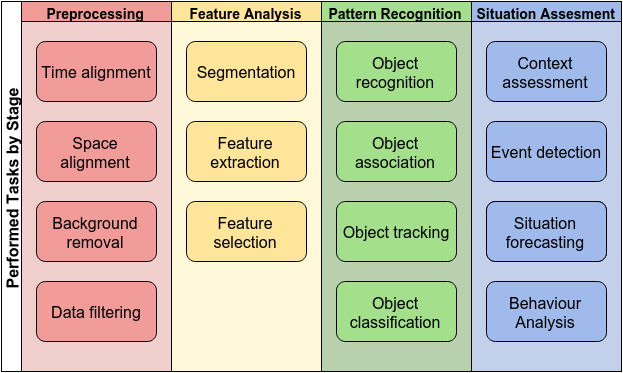
\includegraphics[scale=0.55]{fig/3/processing_stages_and_tasks.png}
\caption{Processing stages in an IMS and commonly performed tasks within each of them}
\label{proc_stages}
\end{figure}


\subsection{Fusion approaches}

Depending on wheter the system has multiple sensors of the same type or different type, a data fusion approach should be chosen. When data came from same-type sensors, it is usually fused at low levels using techniques for temporal-spatial alignment, depending on sensors configuration. This is the case for a network of lasers or lidars or for multi-camera systems. If the system have different type of sensors, data from them may be fused at mid level, based on extracted features or classes on each subsystem; or may be fused at high level if each subsystem delivers control or decision outputs. The tasks shown in each of the processing stages (Figure \ref{proc_stages}), could be used as fusion blocks for homogeneous or heterogeneous data.

\section{Validation approaches}

Before deploying an IMS, it is needed to test some of its components and validate their results. Two commonly used tools for this purpose are traffic simulation models and datasets, depending on the component to be tested. Below, a description of each one is presented.

\subsection{Transportation and Traffic Simulation}

Transportation is a highly complex activity where different elements, like infrastructure, vehicles and pedestrians, affect efficiency, safety and quality of traffic. Intersections are special cases because there exists a high interaction between those mentioned elements making of these places critical points for mobility. For this reason, it is needed to have traffic models to allow the simulation of new policies or deployments intended to enhance transportation.

Three widely-known models for this kind of analysis are macroscopic model, microscopic model and mesoscopic model. The macroscopic model of traffic flow is based on a hydrodynamic analogy, modeling traffic as a fluid process characterized by three main variables, density, volume and speed, and the objective is to describe time-space evolution of those variables.


A more detailed analysis of traffic simulation models and simulation platforms could be found in \cite{AdamsBoxill2000, Barcelo2000, Kitamura2005, Lieberman1992}
\subsubsection{Simulators Classification}
\subsection{Intersection monitoring Datasets}

As mentioned in section \ref{s23}, POSS-i and Ko-PER projects are leading the development of multisensor Intersection Management Systems. One of the contributions of these projects is the creation of datasets of such systems. They provide camera and laser information of a monitored intersection in Peking, China and Aschaffenburg, Germany, respectively. Next, a description of these two datasets will be given.

\subsubsection{POSSi Dataset }

POSSi dataset\footnote{Available at http://www.poss.pku.edu.cn/download.html}
\subsubsection{KoPER Dataset }

Ko-PER dataset\footnote{Available at http://www.uni-ulm.de/in/mrm/forschung/datensaetze.html}

The full description of this dataset is presented in \cite{Strigel2014}.

\section{Architecture proposal}

The proposal presented in this work is based on MFI model processing entities in the sense that a processing block could take one or more inputs related between them and generate an output of the same type or a higher level output. The communication or data exchange approach is based on JDL model, in which data is available over a "bus", where the processing blocks can write to or read from. Four main components of the architecture are defined: communication scheme, data model, information structure and processing blocks. 



\subsection{Communication scheme}

In order to isolate the processing tasks of the communication system, a Publisher-Subscriber approach is selected. The benefits of this option is that data can be shared between diferent blocks without generating a dependency from publishers to subscribers. Another benefit is that exposing a defined mechanism for publishing or subscribing, allows the system to be implementation agnostic.

Taking these reasons into account, Redis is chosen as communication platform. As stated in their website, "Redis is an open source (BSD licensed), in-memory data structure store, used as a database, cache and message broker"\cite{Redis} which support Publisher-Subscriber paradigm, allowing greater scalability and a more dynamic network topology.

For publishers and subscribers to exchange messages, channels are defined with labels using a namespace approach that describe the source of data and the kind of data. For example a channel containing raw data from a laser scanner could be labeled as \texttt{/sensors/range/laser\_1/data/raw}.

Redis is also used as in-memory storage for configuration data that is not part of the processing flow, like sensor parameters, intersection model and control options. This information is loaded into Redis from a JSON file and it is available for any client requiring it.


\subsection{Data Model}

The data model proposed for the system includes the abstraction of the sensing elements and the intersection model. For the sensing elements, a Sensor base class and two derived classes, RangeSensor class and ImageSensor class, are defined. 

The intersection has been modeled as a class with attributes like a label, a Map object, a set of RangeSensors and CameraSensors objects, a set of Leg objects, and a set of Area objects, for inner areas of the intersection. The Map class contains information about the geometry of the intersection and the coordinate system, including a image intended for visualization of configuration and processing.

The sensors sets are composed of zero or more sensor objects, as defined previously. An Area class is defined as having a bounding box and a label	. From this class, a derived class, Leg, is defined for containing additional information about the legs of the intersection, such as heading of the leg, approaching or departure type. In figure \ref{data_model} is shown an UML diagram for the aforementioned classes and their relationships

\begin{figure}[ht!]
\centering
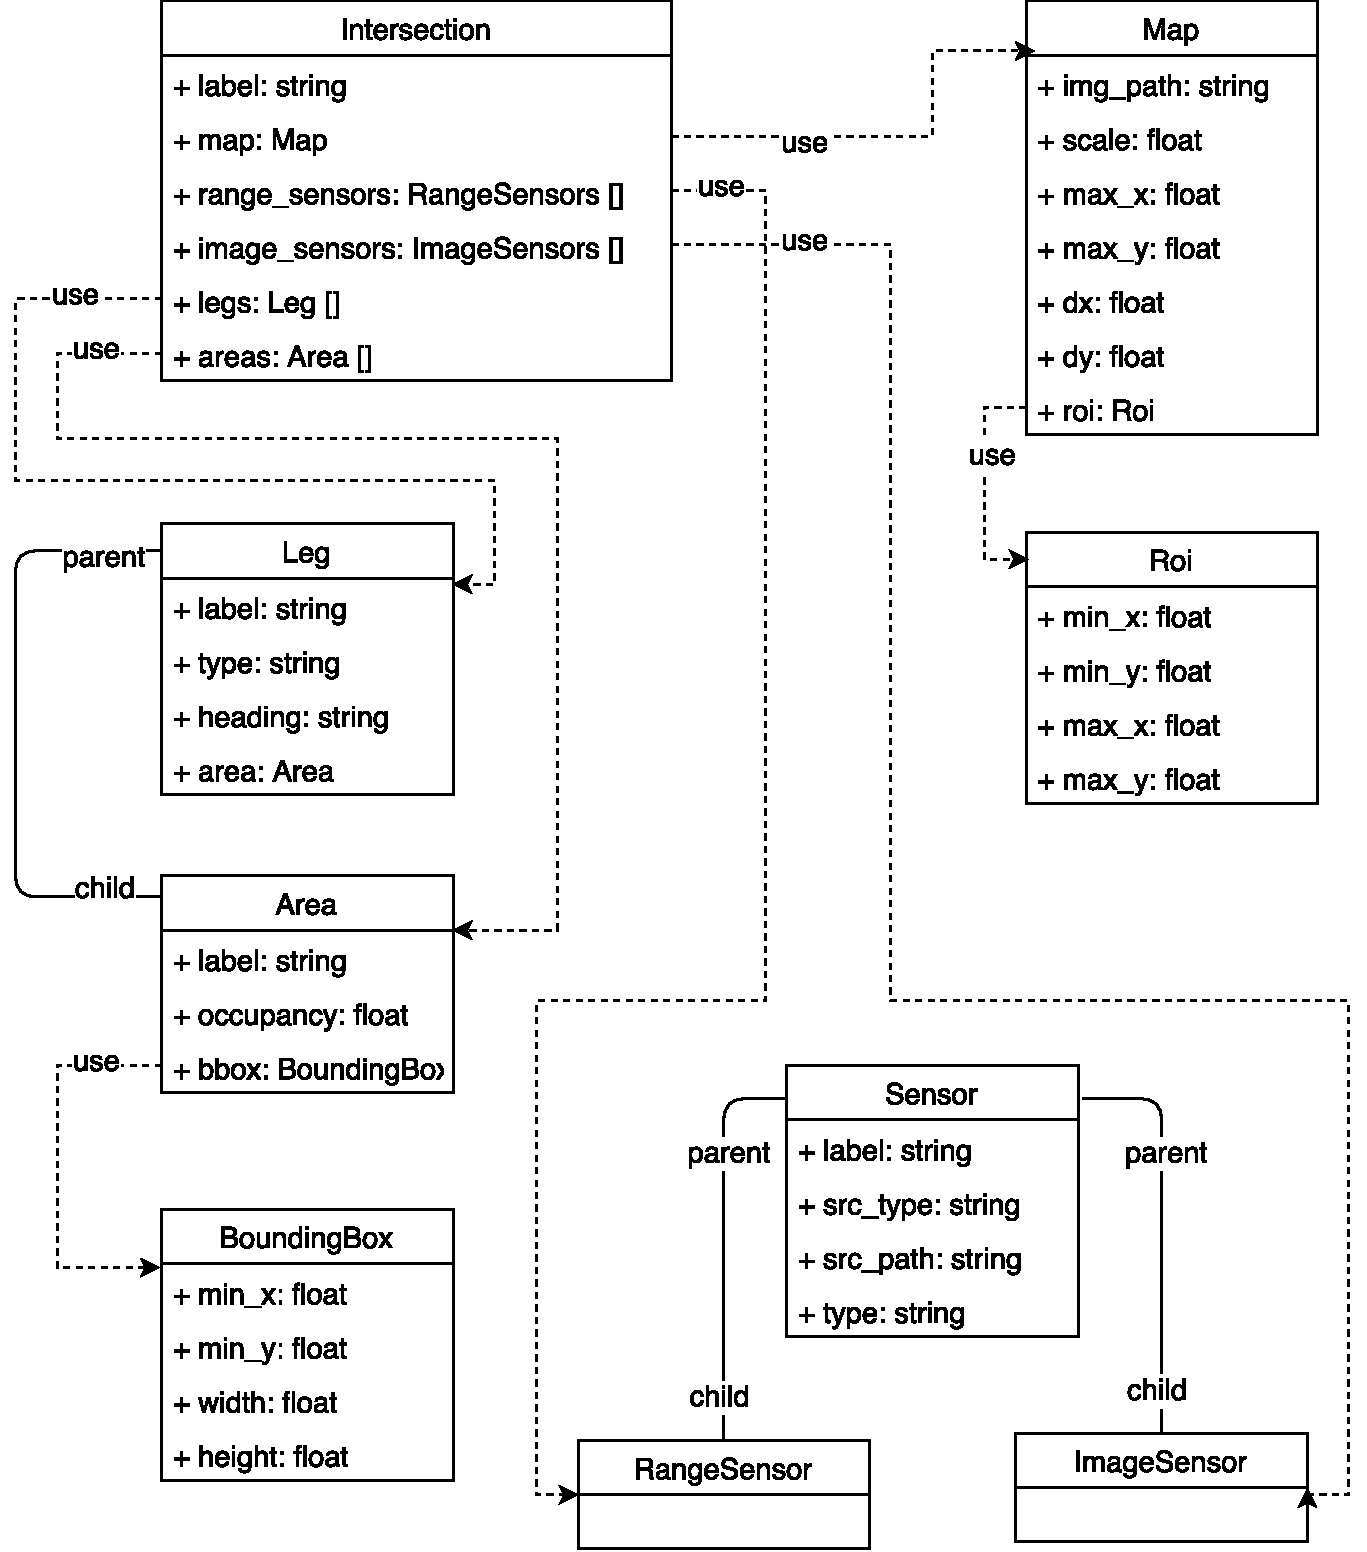
\includegraphics[scale=0.5]{fig/3/data_model.pdf}
\caption{UML diagram of defined entities and their relationships}
\label{data_model}
\end{figure}

The purpose of all the labels attributes within each class is to serve as an identifier of the channel in which the entity is publishing or subscribing to; in other words, to identify where is data generated from or where is data going to. For example, channel \texttt{/sensors/range/laser\_1/data/raw} contains raw data from a laser scanner labeled as \texttt{"laser\_1"} and \texttt{/legs/leg\_3/occupancy/} refers to the occupancy level of the leg labeled as \texttt{leg\_3}.

\subsection{Information Structure}

Data exchanged between processing blocks or any paramater stored in Redis, is formatted using JavaScript Object Notation (JSON), allowing to use any JSON parser/formatter available in many languages, even it is possible to create simple scripts to interact with the system.

\subsubsection{.imscfg file}

For running, the systems requires first a .imscfg file which describes the scenario and the sensors configuration. This information is stored as a JSON object with the properties decribed in table \ref{imscfg_file}.

\begin{table}[ht!]
\footnotesize
\centering
\begin{tabular}{|c | c|}
\hline
\textbf{Property} & \textbf{Description} \\
\hline
name & Name of the configuration \\
\hline
map & Information of the scene, including map, coordinate system \\ 
 & and region of interest. \\
\hline
cameras & List of camera sensors information \\
\hline
range\_sensors & List of range sensors information \\
\hline
legs & List of legs information \\
\hline
intersection & Information of area of the intersection \\
\hline
\end{tabular}
\caption{Properties in .imscfg JSON file}
\label{imscfg_file}
\end{table}

\subsubsection{data messages and configuration parameters}

In addition to .imscfg file, there are different types of messages and parameters which have its own structure, for example used for sensors configuration or processed data. The table \ref{desc_map} gives a description of the types of information used. A more detailed documentation is given in appendix TODO.

\begin{table}[ht!]
\footnotesize
\centering
\begin{tabular}{|c | p{8cm}|}
\hline
\textbf{Name} & \textbf{Description} \\
\hline
laser\_pol\_msg & Contains a timestamp, an array of N angles and and array of N measurements \\
\hline
laser\_cart\_msg & Contains a timestamp, an array of N (x, y) coordinates \\
\hline
laser\_cfg & Contains position and orientation information, also has a background model for the laser sensor \\
\hline
occgrid\_msg & Contains a timestamp and an occupancy grid in the form of an MxN array \\
\hline
\end{tabular}
\caption{Description of diferent types of messages and parameters used}
\label{desc_map}
\end{table}



\subsection{Processing Blocks}

As stated in previous section, there are defined four stages in the processing flow, namely, preprocessing, feature analysis, pattern recognition and situation assessment. Within each of these stages there are different methods and techniques used to process the data and it is possible that those methods are suitable to perform fusion between homogeneous or heterogeneous data.

Below are detailed different processing blocks implemented as part of the whole architecture proposal, classified by the stage of processing in which are located in the process flow. Also, it is shown the format of data input, data output and parameters needed for configuration and execution.

Additionaly, there are included some tools and generic blocks used for dataset reading, data visualization and interactive control.

\subsubsection{Preprocessing}
\begin{description}
\item[laser\_background\_remove]laser\_bg\_remove
\begin{figure}[ht!]
\centering
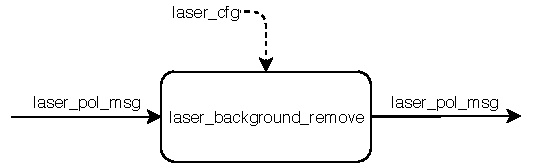
\includegraphics[scale=0.7]{fig/3/laser_bg_remove.pdf}
\caption{laser\_bg\_remove}
\label{laser_bg_remove}
\end{figure}

\begin{figure}[ht!]
\centering
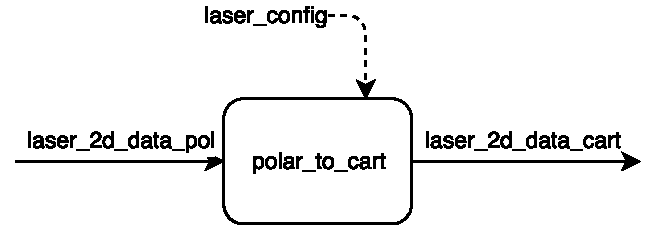
\includegraphics[scale=0.7]{fig/3/polar2cart.pdf}
\caption{polar\_to\_cartesian}
\label{polar_to_cartesian}
\end{figure}

\begin{figure}[ht!]
\centering
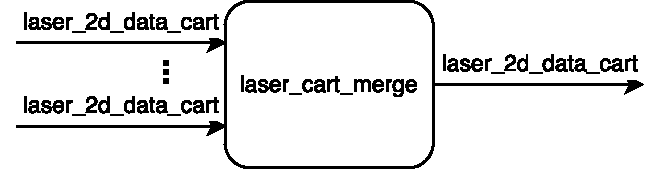
\includegraphics[scale=0.7]{fig/3/laser_cart_merge.pdf}
\caption{laser\_cart\_merge}
\label{laser_cart_merge}
\end{figure}

\begin{figure}[ht!]
\centering
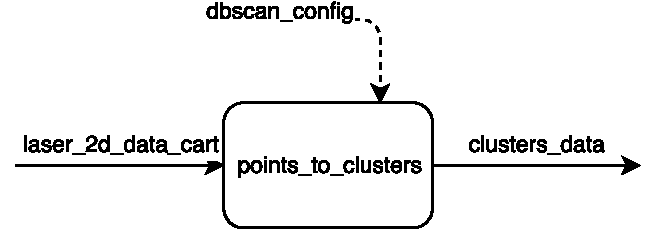
\includegraphics[scale=0.7]{fig/3/points_to_clusters.pdf}
\caption{points\_to\_clusters}
\label{points_to_clusters}
\end{figure}

\begin{figure}[ht!]
\centering
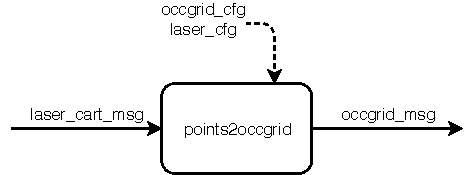
\includegraphics[scale=0.7]{fig/3/points_to_grid.pdf}
\caption{points\_to\_grid}
\label{points_to_grid}
\end{figure}

\begin{figure}[ht!]
\centering
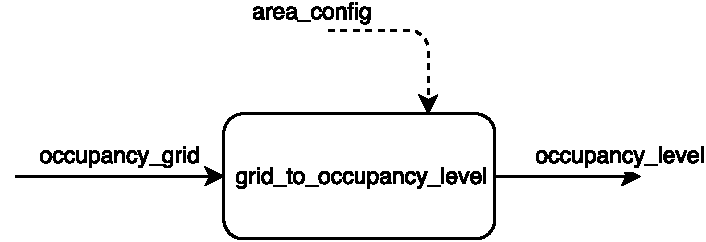
\includegraphics[scale=0.7]{fig/3/grid_to_occupancy_level.pdf}
\caption{grid\_to\_occupancy\_level}
\label{grid_to_occupancy_level}
\end{figure}

\begin{figure}[ht!]
\centering
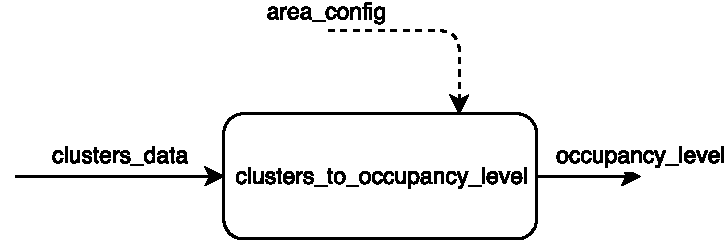
\includegraphics[scale=0.7]{fig/3/clusters_to_occupancy_level.pdf}
\caption{clusters\_to\_occupancy\_level}
\label{clusters_to_occupancy_level}
\end{figure}

\begin{figure}[ht!]
\centering
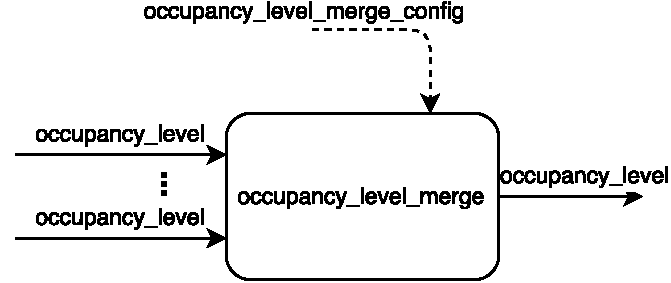
\includegraphics[scale=0.7]{fig/3/occupancy_level_merge.pdf}
\caption{occupancy\_level\_merge}
\label{occupancy_level_merge}
\end{figure}

\begin{figure}[ht!]
\centering
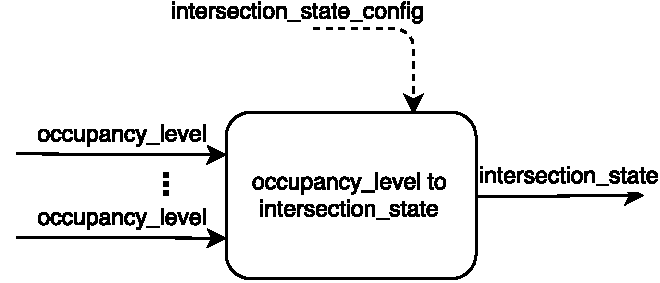
\includegraphics[scale=0.7]{fig/3/occupancy_level2int_state.pdf}
\caption{occupancy\_level\_to\_intersection\_state}
\label{occupancy_level2int_state}
\end{figure}

\end{description}



%{laser_background_remove}
\subsubsection{Feature Analysis}
\subsubsection{Pattern Recognition}
\subsubsection{Situation Assesment}
\subsubsection{Tools and Utilities}